\section{Bandit feedback in Passive-Aggressive bound (BPA)}
\label{subsec:BPA}
Different to the PAB algorithm, \text{BPA} \cite{zhong2015passive} also an adaptation of PA, but its error has a same bound as PA. Similar to PAB, at each round it outputs a prediction $\hat{y}_t$ to be the label with the highest score of $\left\langle w_i,x_t\right\rangle$, is defined as below:
\begin{equation}
\hy = h_t(x_t) = \underset{i\in \{1,\dots,K\}}{\text{argmax}}\left\langle w_i,x_t\right\rangle
\end{equation}
where $w_i\in \Rd$ is the $i^{th}$ row of the matrix $w\in \RKd$. 
Unlike the conventional learning paradigm, if $\hy\neq y_t$ algorithm PA to be difficult to get update because the true label's information is not supported by the bandit setting. 
So it need to perform an exploration, i.e., sample a label randomly $[k]$ with parameter $\gamma$ and contrast this random prediction with a bandit return $\1_{\tilde{y}_t = y_t}$, 
where $\tilde{y}_t$ is the result of a random draw from a certain distribution $\mathbb{P}(\tilde{Y}|\hy)$ by $\epsilon$-Greedy Algorithm~\ref{algo:epsilon}. Here gives an instantaneous loss by the following function,
\begin{equation}
\label{equa:BPAloss}
l_t = [1+\left(1-2\1_{\tilde{y}_t=y_t}\right)\left\langle w_{\tilde{y}_t},x_t\right\rangle]_{+}
\end{equation}
with $\left(1-2\1_{\tilde{y}_t=y_t}\right)$ equal to -1 when $\tilde{y}_t = y_t$ and 1 elsewhere. 
This loss is the standard hinge loss when the prediction is correct: it stays at 0 for $\left\langle w_{\tilde{y}_t},x_t\right\rangle \geqslant 1$ and then increases for decreasing values of $\left\langle w_{\tilde{y}_t},x_t\right\rangle$. 
In contrast, when the prediction is incorrect, the loss is equal to $[1+\left\langle w_{\tilde{y}_t},x_t\right\rangle]_{+}$, 
i.e., stays at 0 for $\left\langle w_{\tilde{y}_t},x_t\right\rangle\leq -1$ 
and then increases for increasing values of $\left\langle w_{\tilde{y}_t},x_t\right\rangle$.

The linear classifiers are updated at each trial using the standard tools from convex analysis\cite{Boyd04}, Where $w_t$ satisfies the constraint in Eq.~\ref{equa:paconstraint}.

\begin{equation}
\label{equa:pablagrangian}
L(w,\tau) = \frac{1}{2}\parallel{w-w_t}\parallel^2 + \tau \left(1+ (1-2\1_{\tilde{y}_t=y_t})\left\langle w_{\tilde{y}_t},x_t\right\rangle\right)
\end{equation}

\begin{equation}
\label{equa:BPAupdate}
w_{t+1} = w_t + \tau \left(2\1_{\tilde{y}_t = y_t}-1\right) \Phi(x_t,\tilde{y}_t)
\end{equation}

Taking the derivative of $L(\tau)$ with respect to $\tau$ and also setting it to zero, we get that:
\[ \tau = \frac{l_t}{\parallel{\Phi(x_t,\ty)}\parallel^2}\]

Considering for instance the common phenomenon of label noise, a mislabeled example may cause PA to drastically change its classifiers in the wrong direction. To derive soft-margin classifiers \cite{vapnik1998statistical} and a non-negative slack variable $\xi$ is introduced into the optimization problem in Equation~\ref{equa:paconstraint}. According with \cite{crammer2006online}, the variable can be introduced in two different ways.
\[
\left\{
\begin{matrix}
w_{t+1} = \underset{w\in \mathbb{R}^{K\times d}}{argmin}\frac{1}{2}\parallel{w-w_t}\parallel^2 + C\xi    & \text{s.t.  }  l(w;(x_t,y_t))\leqslant \xi \ and\ \xi \geqslant 0 \\ 
w_{t+1} = \underset{w\in \mathbb{R}^{K\times d}}{argmin}\frac{1}{2}\parallel{w-w_t}\parallel^2 + C\xi^2 & \text{s.t.  }  l(w;(x_t,y_t))\leqslant \xi
\end{matrix}
\right.
\]
By these optimization problems, we get the corresponding optimization solutions:
\[
\left\{
\begin{matrix}
w_{t+1} = w_t + (2 \delta_{(\ty =y_t)}-1)\cdot \text{min}\left\{C, \frac{l_t}{\parallel{\Phi(x_t,\ty)}\parallel^2}\right\} \cdot \Phi(x_t,\ty) \\
w_{t+1} = w_t + (2 \delta_{(\ty =y_t)}-1)\cdot \frac{l_t}{\parallel{\Phi(x_t,\ty)}\parallel^2+\frac{1}{2C}} \cdot \Phi(x_t,\ty)
\end{matrix}
\right.
\]

%!ALGORITHM-----------------------------
%!--------------------------------------
\begin{algo}[Bandit Passive-Aggressive]
%\caption{BPA}
\begin{algorithmic}
\STATE $\ \ $
\STATE Parameter: number $\gamma\in \left(0,1\right)$.
\STATE Initialize: Set $W_1$ to the zero $K \times d$ matrix.
\FOR {each round t = 1,2,\dots, n}
	\STATE Observe $x_t \in \Rd$.
    \STATE Set $\hy = \underset{i = 1,\dots,K}{argmax}\left\langle W_t^i ,x_t\right\rangle$
    \FORALL {$i \in [K]$}
    	\STATE $\mathbb{P}(\tilde{Y} = i | \hy) = (1-\gamma)\1_{i = \hy} + \frac{\gamma}{K}$
    \ENDFOR
    \STATE Draw $\tilde{y}_t$ randomly from distribution $p_t = \left(p_{1,t},\dots ,p_{K,t}\right)$.
    \STATE Observe $\1_{(\hy=y_t)}$.
    \STATE $l_t = [\1_{\ty=y_t}+(1-2\1_{\tilde{y}_t=y_t})\left\langle w_{t,\tilde{y}_t},x_t\right\rangle]_{+}$
    \STATE Update $W_{t+1} = W_t + (2\1_{\tilde{y}_t=y_t}-1)\frac{l_t}{\parallel{x_t}\parallel^2}\cdot\Phi(x_t,\tilde{y}_t)$.
\ENDFOR
\end{algorithmic}
\end{algo}
%!----------------------------------------
\subsection{Analysis}
\label{subsec:BPAA}
In this section, we prove the cumulative squared loss has a upper bound. To simplify, we note $l(w_t;(x_t,y_t))$ as $l_t$ and $l(u;(x_t,y_t))$ as $l_t^{\ast}$.
\begin{theo}
\label{theo:BPAT1}
Let $(x_1,y_1),...,(x_T,y_T)$ be a sequence of separable examples where $x_t \in \\mathbb{R}^d$, $y_t\in \mathscr{Y}$ and $\parallel{x_t}\parallel\leqslant R$ for all t, and $u \in \mathbb{R}^{K\times d}$. Then, the cumulative squared loss of this algorithm is bounded by,
\begin{equation}
\sum_{t=1}^{T} l_t^2 \leqslant R^2\cdot \parallel{u}\parallel^2
\end{equation}
\end{theo}

\begin{proof}
Define $\Delta_t$ to be:
\[\Delta_t = \parallel{w_t-u}\parallel^2-\parallel{w_{t+1}-u}\parallel^2\]
By summing $\Delta_t$ over all t from 1 to T, that $\sum_t \Delta_t$ is a telescopic sum which collapses to,
\[\sum_{t=1}^{T}\Delta_t = \sum_{t=1}^{T} \left( \parallel{w_t - u}\parallel^2-\parallel{w_{t+1} - u}\parallel^2 \right) = \parallel{w_1 - u}\parallel^2-\parallel{w_{t+1}-u}\parallel^2\]
By the initiation of $w_1 = \vec{0}$, 
\begin{equation}
\label{equa:delta}
\sum_{t=1}^{T}\Delta_t = \parallel{u}\parallel^2 - \parallel{w_{t+1}-u}\parallel^2 \leqslant \parallel{u}\parallel^2 
\end{equation}

Using the definition of update in Eq.\ref{update},
\[\Delta_t = -2\left< (w_t - u), (2\delta-1)\frac{l_t}{\parallel{\Phi(x_t,\ty)}\parallel^2}\Phi(x_t,\ty)\right> - \left( \frac{l_t}{\parallel{\Phi(x_t,\ty)}\parallel^2}\Phi(x_t,\ty)\right)^2\]
With  $l_t = [1+(1-2\delta_{(\tilde{y}_t = y_t)})\cdot\langle w_t,\Phi(x_t,\ty)\rangle]_+$  and  $l_t^{\ast} = [1+(1-2\delta_{(\tilde{y}_t = y_t)})\cdot\langle w^{\ast},\Phi(x_t,\ty)\rangle]_+$ ,
So, 
\[\Delta_t = 2\frac{l_t^2 - l_t l_t^{\ast}}{\parallel{\Phi(x_t,\ty)}\parallel^2}-\left( \frac{l_t}{\parallel{\Phi(x_t,\ty)}\parallel^2}\parallel{\Phi(x_t,\ty)}\parallel \right)^2\]
\[\Delta_t = \frac{l_t^2-2l_t l_t^{\ast}}{\Phi(x_t,\ty)\parallel^2}\]
If all examples are separable, $\exists u$ such that $\forall t \in [1,...,T]$ , $l_t^{\ast} = 0$, following the Eq.~\ref{sumDelta},

\[\Rightarrow \parallel{u}\parallel^2 \geqslant \sum_{t=1}^{T}\Delta_t \geqslant \sum_{t=1}^{T} \left( \frac{l_t^2}{\parallel{\Phi(x_t,\ty)}\parallel^2}\right)\]
\[\Rightarrow \sum_{t=1}^{T} l_t^2 \leqslant\parallel{u}\parallel^2 \cdot \parallel{\Phi(x_t,\ty)}\parallel^2\]
\[\sum_{t=1}^{T} l_t^2 \leqslant R^2 \cdot \parallel{u}\parallel^2\]
\end{proof}
\begin{theo}
\label{theo:BPAT2}
Let $(x_1,y_1),...,(x_T,y_T) $ be a sequence of non-separable examples where  $x_t\in \mathbb{R}^d$, $y_t \in [k]$ and $\parallel{x_t}\parallel \leqslant R$ for all t. Then for any vector $u \in \mathbb{R}^{K\times d}$ the cumulative squared loss of this algorithm is bounded by:
\[\sum_{t=1}^{T}l_t^2 \leqslant \left(R\parallel{u}\parallel+2 \sqrt{\sum_{t=1}^{T}(l_t^{\ast})^2}\right)^2 \]
\end{theo}
\begin{proof}
By the proof of Theorem \ref{theo:BPAT1}, 
\[\sum_{t=1}^{T}l_t^2 \leqslant R^2\cdot \parallel{u}\parallel^2 + 2\sum_{t=1}^{T}l_t l_t^{\ast}\]
To upper bound the right side of the above inequality, and denotes $L_t = \sqrt{\sum_{t=1}^{T}l_t^2}$ and $U_t = \sqrt{\sum_{t=1}^{T}(l_t^{\ast})^2}$, 
\[2(L_tU_t)^2-2(\sum_{t=1}^{T}l_tl_t^{\ast})^2 = \sum_{i=1}^{T}\sum_{j=1}^{T}l_i^2(l_j^{\ast})^2+\sum_{i=1}^{T}\sum_{j=1}^{T}l_j^2(l_i^{\ast})^2 - 2\sum_{i=1}^{T}\sum_{j=1}^{T}l_il_jl_i^{\ast}l_j^{\ast}\]
\[ = \sum_{i=1}^{T}\sum_{j=1}^{T}(l_il_j^{\ast}-l_jl_i^{\ast})^2 \geqslant 0\]
\[\sum_{t=1}^{T}l_t^2 \leqslant R^2 \cdot \parallel{u}\parallel^2+2\sum_{t=1}^{T}l_tl_t^{\ast}\leqslant R^2 \cdot \parallel{u}\parallel^2+2L_tU_t\]
%\[L_t^2 -2R^2 L_tU_t+U_t^2\leqslant R^2\parallel{u}\parallel^2+U_t^2\]
\[L_t \leqslant U_t+\sqrt{R^2\parallel{u}\parallel^2+U_t^2}\]
Using the fact that $\sqrt{a+b}\leqslant \sqrt{a}+\sqrt{b}$,
\[L_t \leqslant R\parallel{u}\parallel+2 U_t\]
\[\sum_{t=1}^{T}l_t^2 \leqslant \left(R\parallel{u}\parallel+2 \sqrt{\sum_{t=1}^{T}(l_t^{\ast})^2}\right)^2 \]
\end{proof}

\subsection{Experiment}
\label{subsec:BPAE}
Here, we evaluate the algorithms over two synthetic and three real world data sets. Their characteristics are summarized in Table~\ref{table:mce}.

\begin{table}[b]
\caption{Summary of the five data sets, including the numbers of instances, features, labels and whether the number of examples in each class are balanced.}
\label{table:mce}
\begin{center}
\begin{tabular}{|c|c|c|c|c|}
\hline 
Data           & Instances 	&Features 	&  Labels 	& Balanced\\ 
\hline 
SynSep         &100 000 	& 400   	& 9  		& Y \\
\hline 
SynNonSep      &100 000 	& 400   	& 9  		& Y \\
\hline 
RCV1-v2        &100 000 	& 47236 	& 53 		& N \\
\hline 
Letter         &20 000  	& 16    	& 26 		& N \\
\hline 
Pen-Based &13 200  	& 16    	& 10 		& N \\
\hline 
\end{tabular}
\end{center}
\end{table}

\textbf{Data sets}:
The first data set, denoted by SynSep,  is a 9-class, 400-dimensional synthetic data set of size $10^5$. More details about the method to generate this data set can be found in \cite{kakade2008efficient}. The SynSep  idea is to have a simple simulation of generating a text document. The coordinates represent different words in a small vocabulary of size $400$. We ensure that SynSep is linearly separable. 

The second data set, denoted by SynNonSep, is constructed  the same way as  SynSep except that a 5\% label noise is introduced, which makes the data set non-separable. 

The third data set is collected from the Reuters RCV1-v2 collection\cite{David04RCV}. The original data set is composed by multi-label instances. So we make some preprocessing likes \cite{RB08a}. First, its label hierarchy is reorganized by mapping the data set to the second level of RCV1 topic hierarchy. The documents that have labels of the third or forth level only are mapped to their parent category of the second level; Second, all multi-labelled instances have been removed. This RCV1-v2 is a 53-class,  47236-dimensional real data set of size $10^5$. 

The fourth and fifth data sets are collected from \cite{letter26SC,number10SC}. The fourth data set is to identify each of a large number of black-and-white rectangular pixel displays as one of the 26 capital letters in the English alphabet. The character images were based on 20 different fonts and each letter within these 20 fonts was randomly distorted to produce a file of 20000 unique stimuli. Each stimuli was converted into 16 primitive numerical attributes (statistical moments and edge counts). It forms a 26-class, 16-dimensional real data set of size $20000$. The fifth data set is a digit data base made by collecting 250 samples from 44 writers, using only (x,y) coordinate information represented as constant length feature vectors, which were resampled to 8 points per digit (therefore the data set contains 8 points $\times$ 2 coordinates = 16 features). This one is a 10-class, 16-dimensional real data set of size $10992$.

\textbf{Results}
Figures \ref{pic:BPASS} and \ref{pic:BPASNS} show the experimental results on two synthetic data sets and three real data sets. For SynSep, a separable linear data set, all algorithms except Banditron obtain a good performance; with the non-separable SynNonSep data, Confidit and BPA outperform the other algorithms, even the algorithms having a full feedback.

With the three real data sets, the algorithms with full information, despite their competitive advantage with respect to the ones with bandit feedback, do not significantly depart from BPA and Confidit, with classification results that clearly outperform Banditron. While having a lower computational complexity, BPA approach is even found to outperform Confidit in the most challenging situation, i.e. the high-dimensional case with a large number of classes (RCV1-v2 data set).

The $\gamma$ parameter represents the exploration rate in Banditron and BPA algorithms. We compare on Figure 3 the average error rates obtained on the two algorithms for different values of $\gamma$ on the different data sets. In contrast with Banditron, BPA shows that $\gamma$ has a very little influence on the final error rate, indicating a capability to deal with small exploration rates.


\begin{figure}[h!]

\centerline{
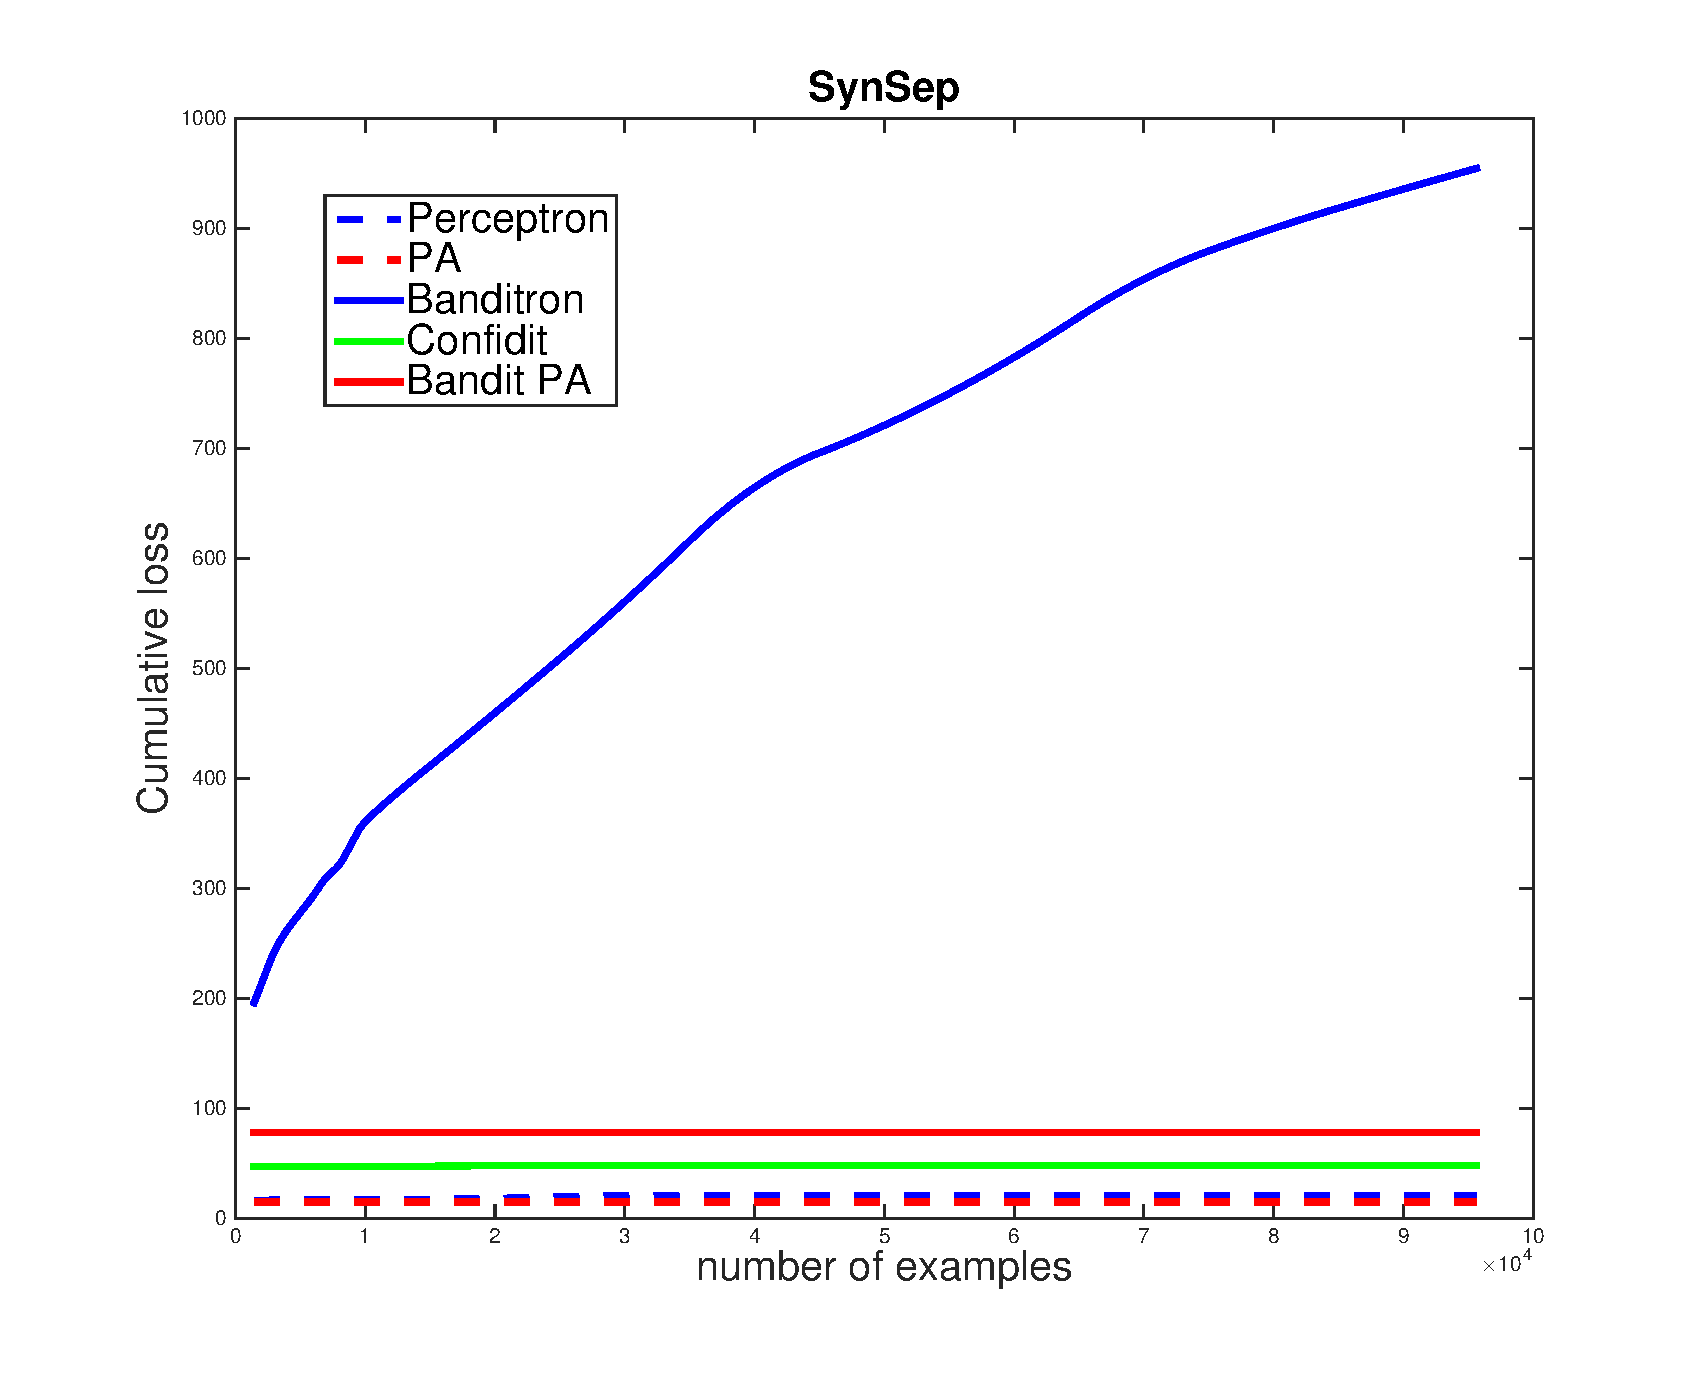
\includegraphics[scale = 0.4]{fig05/mc/SynSep.eps}
}
\caption{Cumulative Errors on the synthetic data set of  SynSep.}
\label{pic:BPASS}
\end{figure}
\begin{figure}[h!]

\centerline{
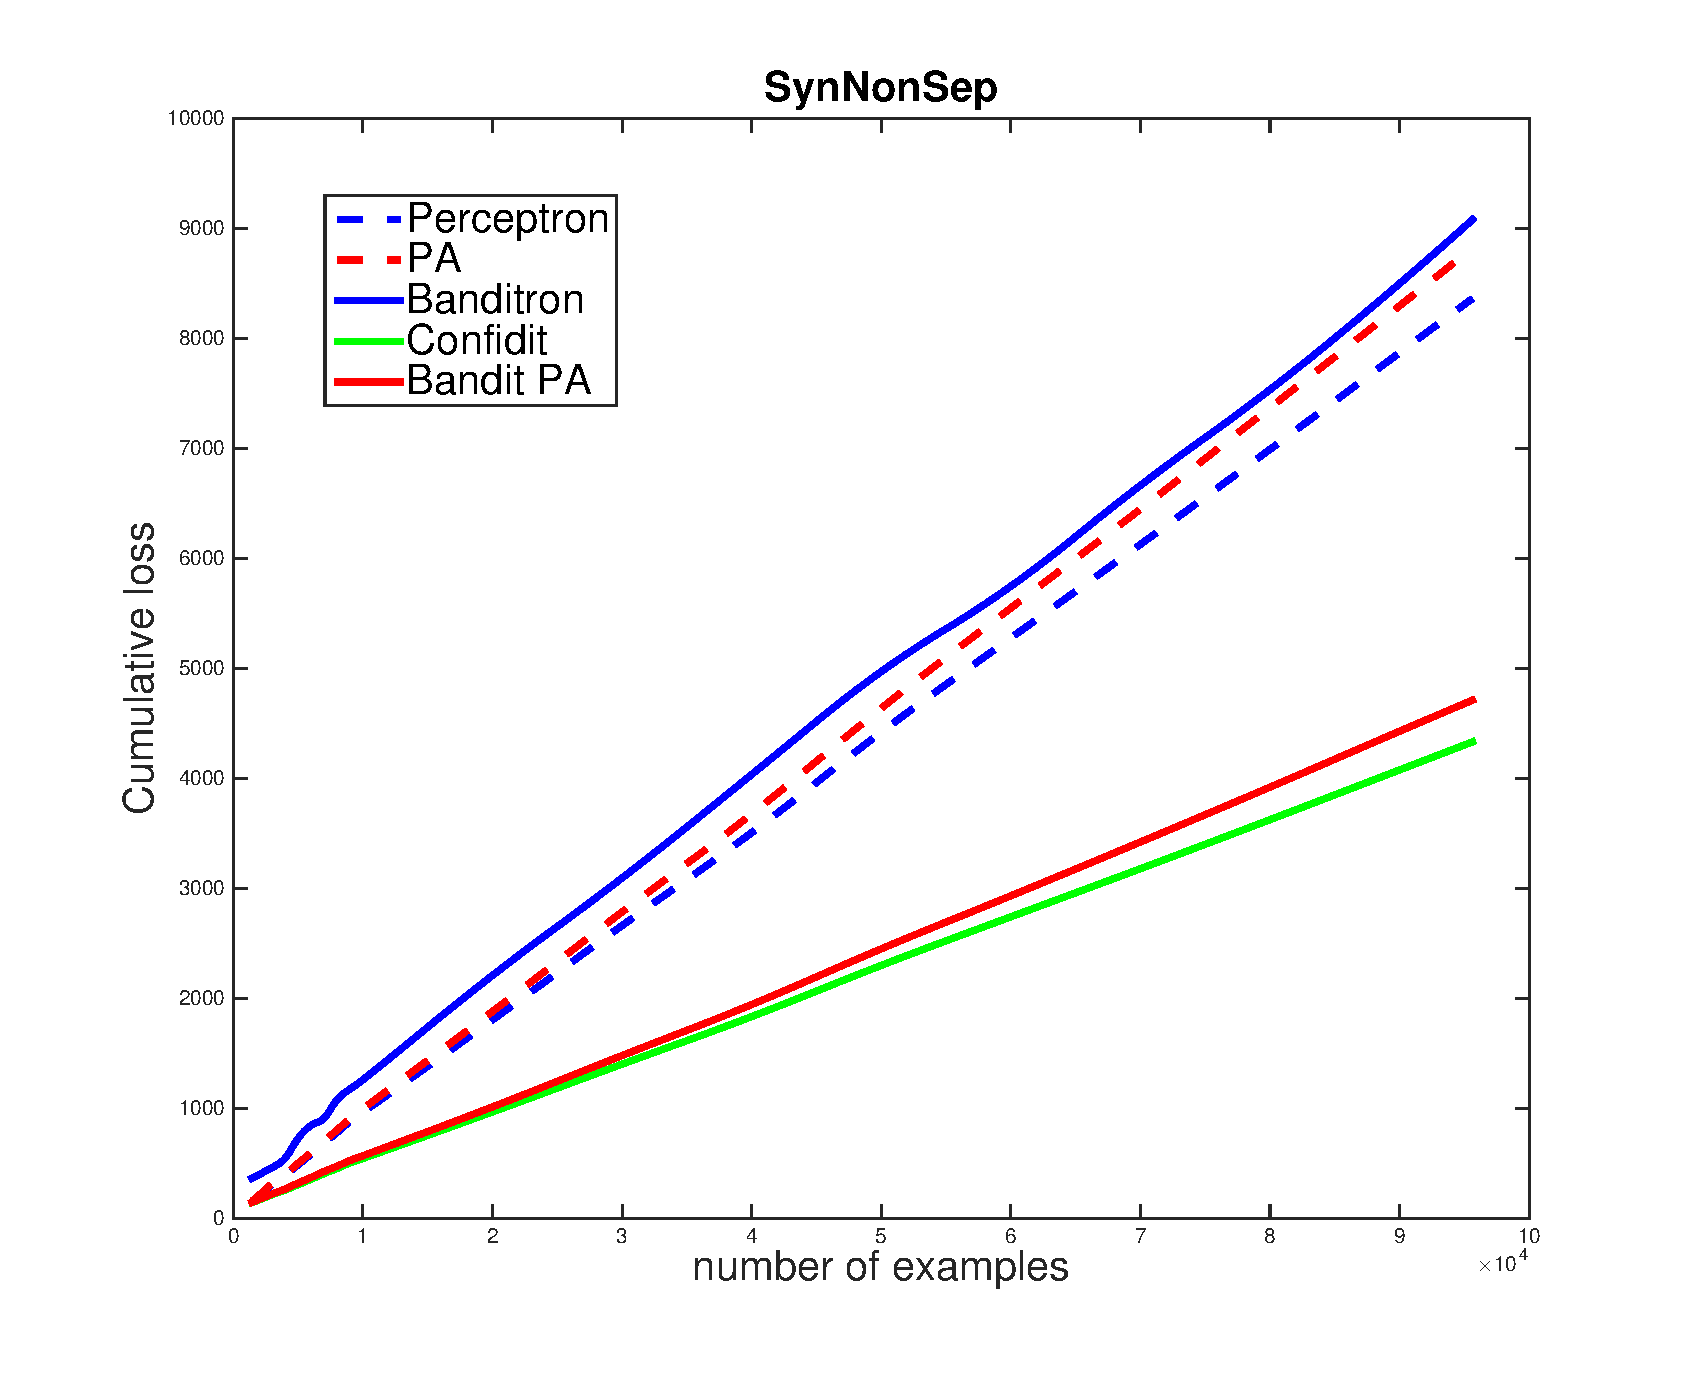
\includegraphics[scale = 0.4]{fig05/mc/SynNonSep.eps}
}
\caption{Cumulative Errors on the synthetic data set of SynNonSep.}
\label{pic:BPASNS}
\end{figure}
\begin{figure}[h!]
\label{pic:BPARCV}
\centerline{
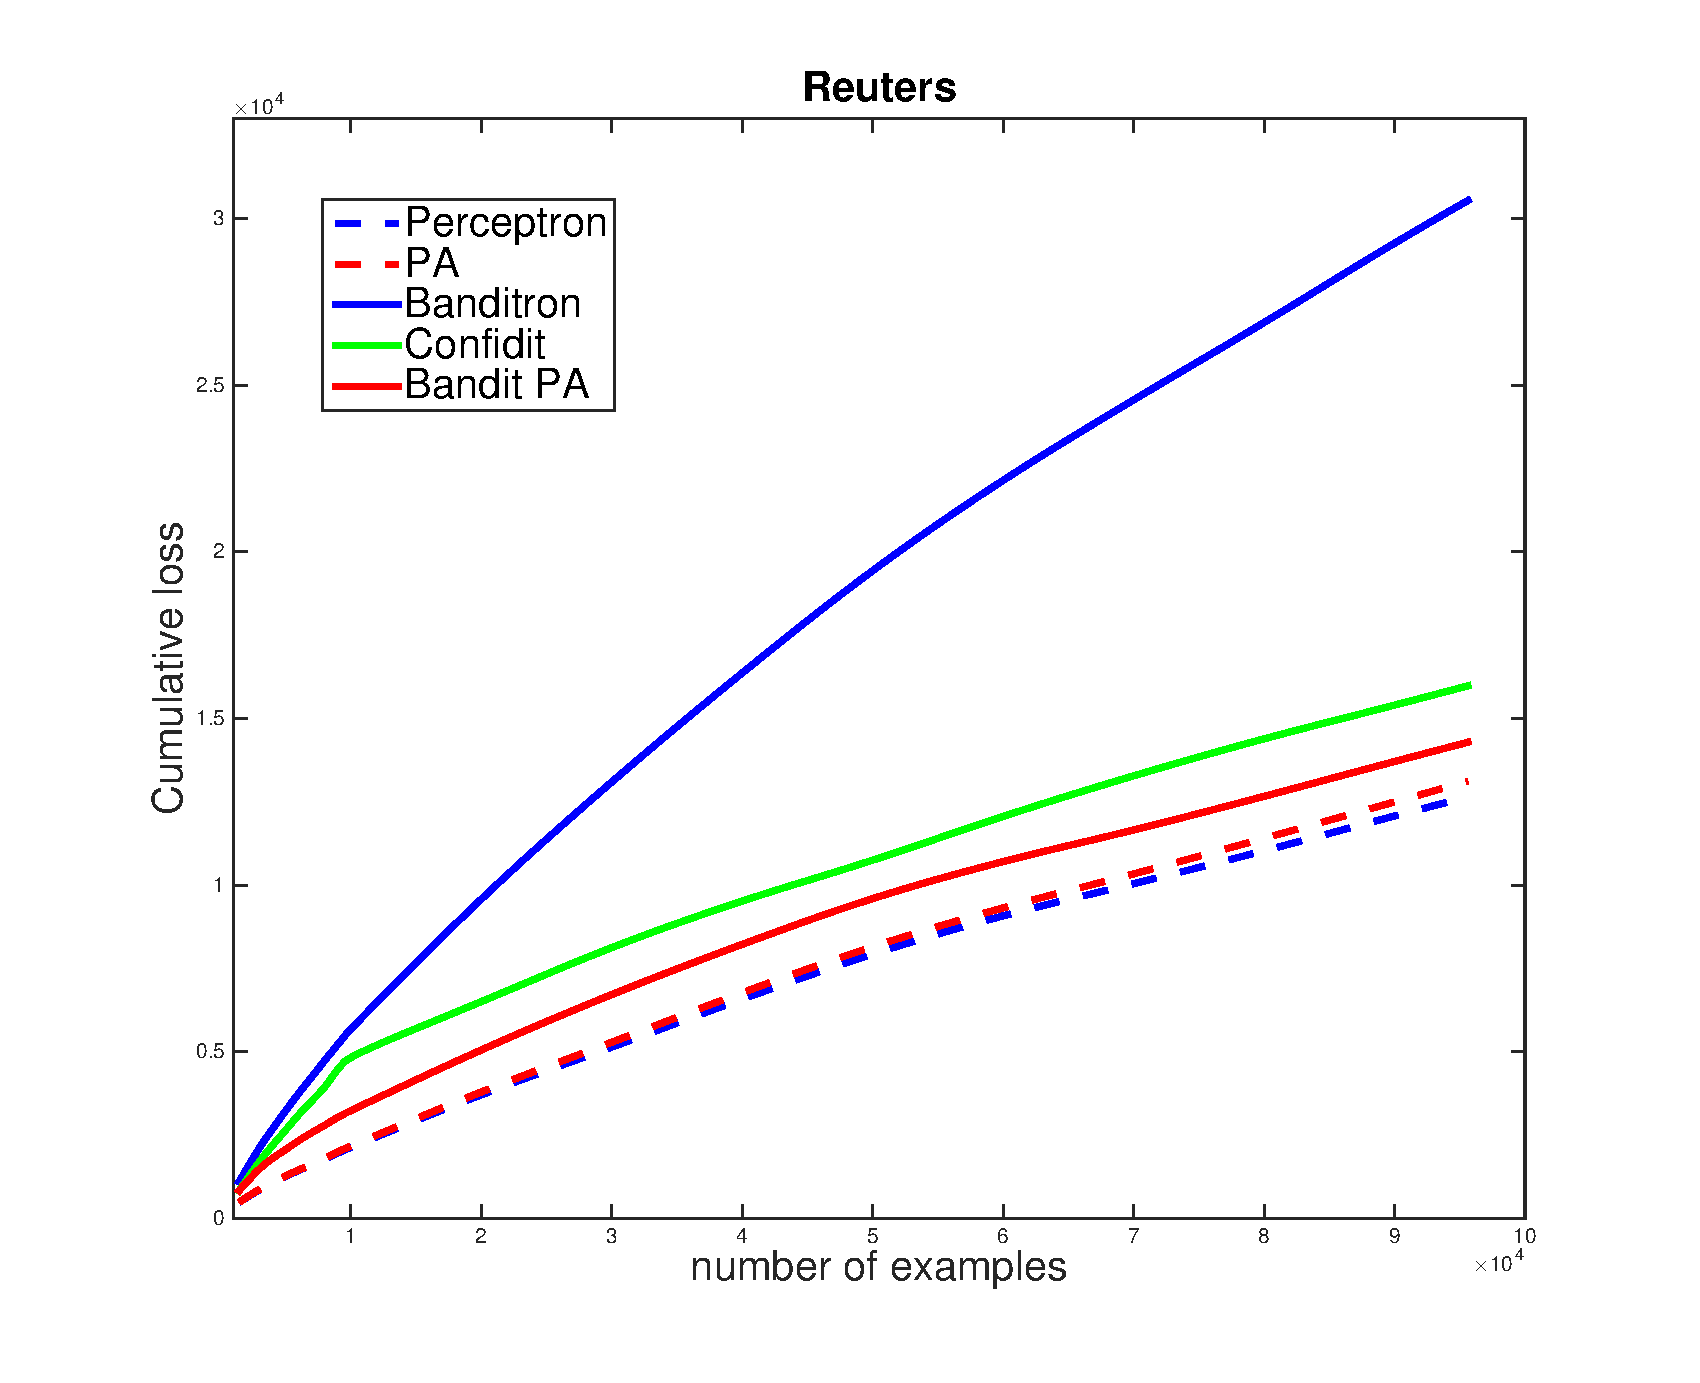
\includegraphics[scale = 0.4]{fig05/mc/RCV1_v2_53class.eps}}
\caption{Cumulative Errors on the real data set of RCV1-v2 (53 classes).}
\end{figure}

\begin{figure}[h!]
\centerline{
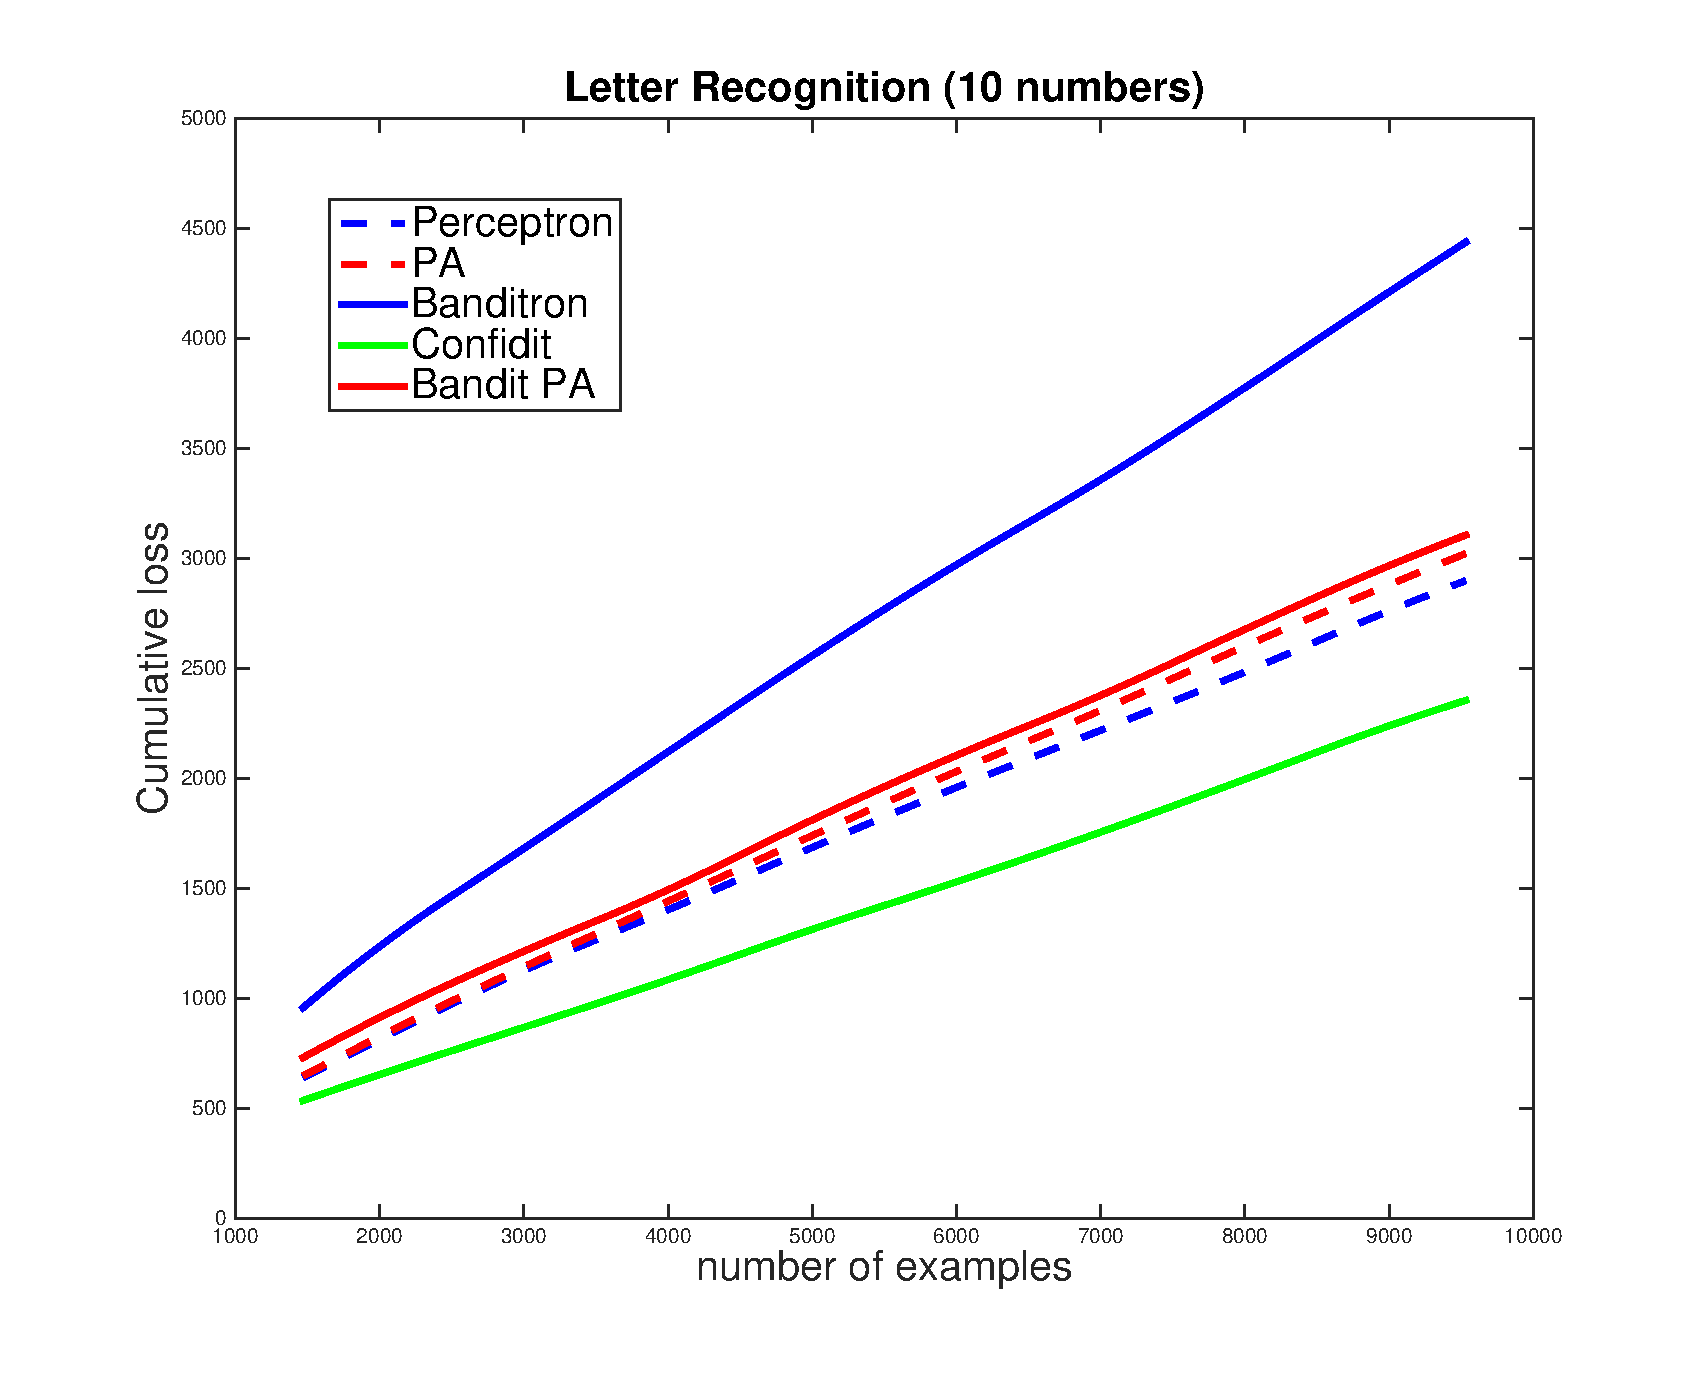
\includegraphics[scale = 0.4]{fig05/mc/10LR.eps}}
\caption{Cumulative Errors on the real data set of Letter Recognition (10 numbers).}
\label{pic:BPALR10}
\end{figure}

\begin{figure}[h!]
\centerline{
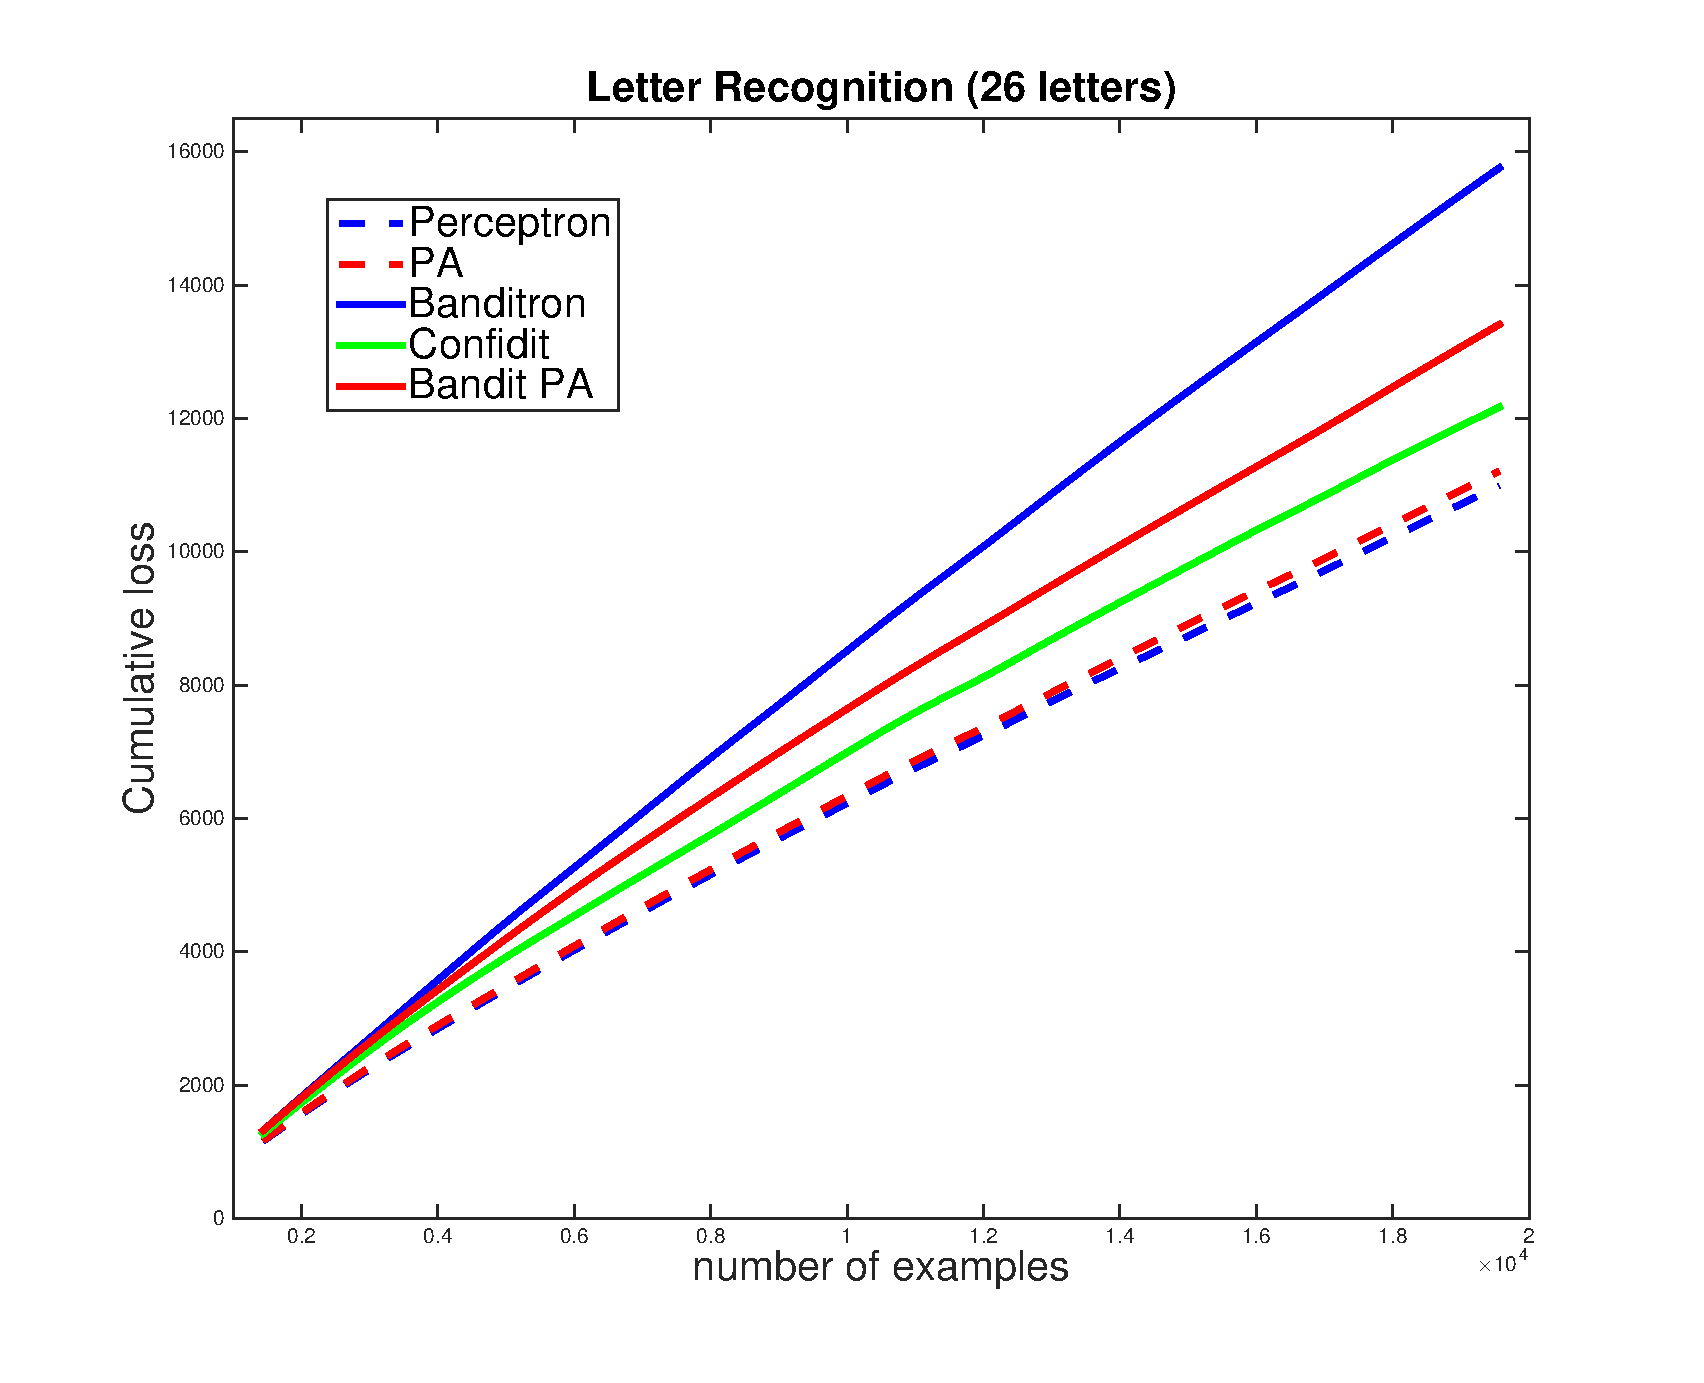
\includegraphics[scale = 0.4]{fig05/mc/26LR.eps}}
\caption{Cumulative Errors on the real data set of Letter Recognition (26 Letters).}
\label{pic:BPALR26}
\end{figure}

\begin{figure}[h!]
\centerline{
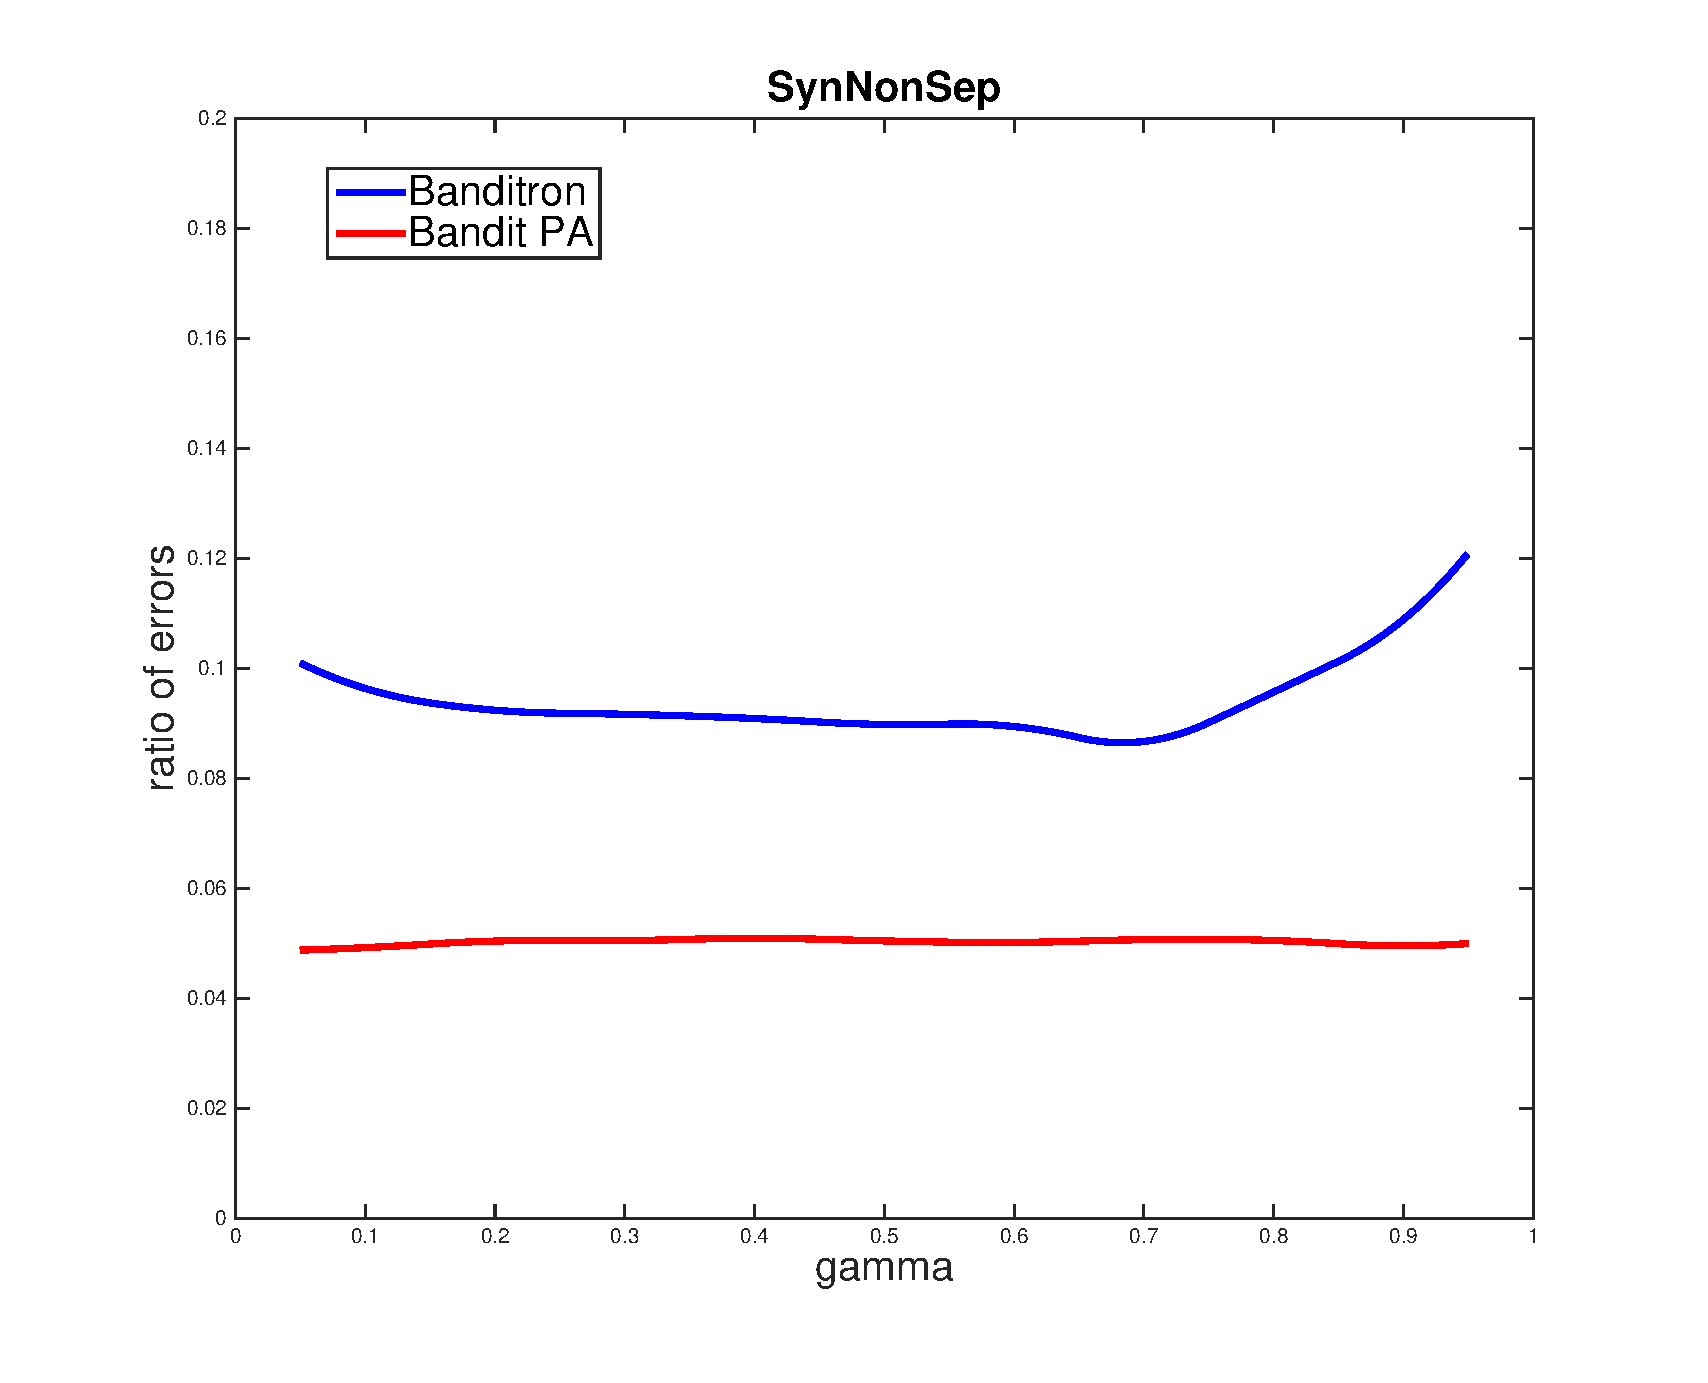
\includegraphics[scale = 0.4]{fig05/mc/SynNonSep_gamma.eps}}
\caption{Average error of Banditron and BPA for parameter's value $\gamma$ on the data set of SynNonSep.}
\label{pic:BPASNSerr}
\end{figure}

\begin{figure}[h!]
\centerline{
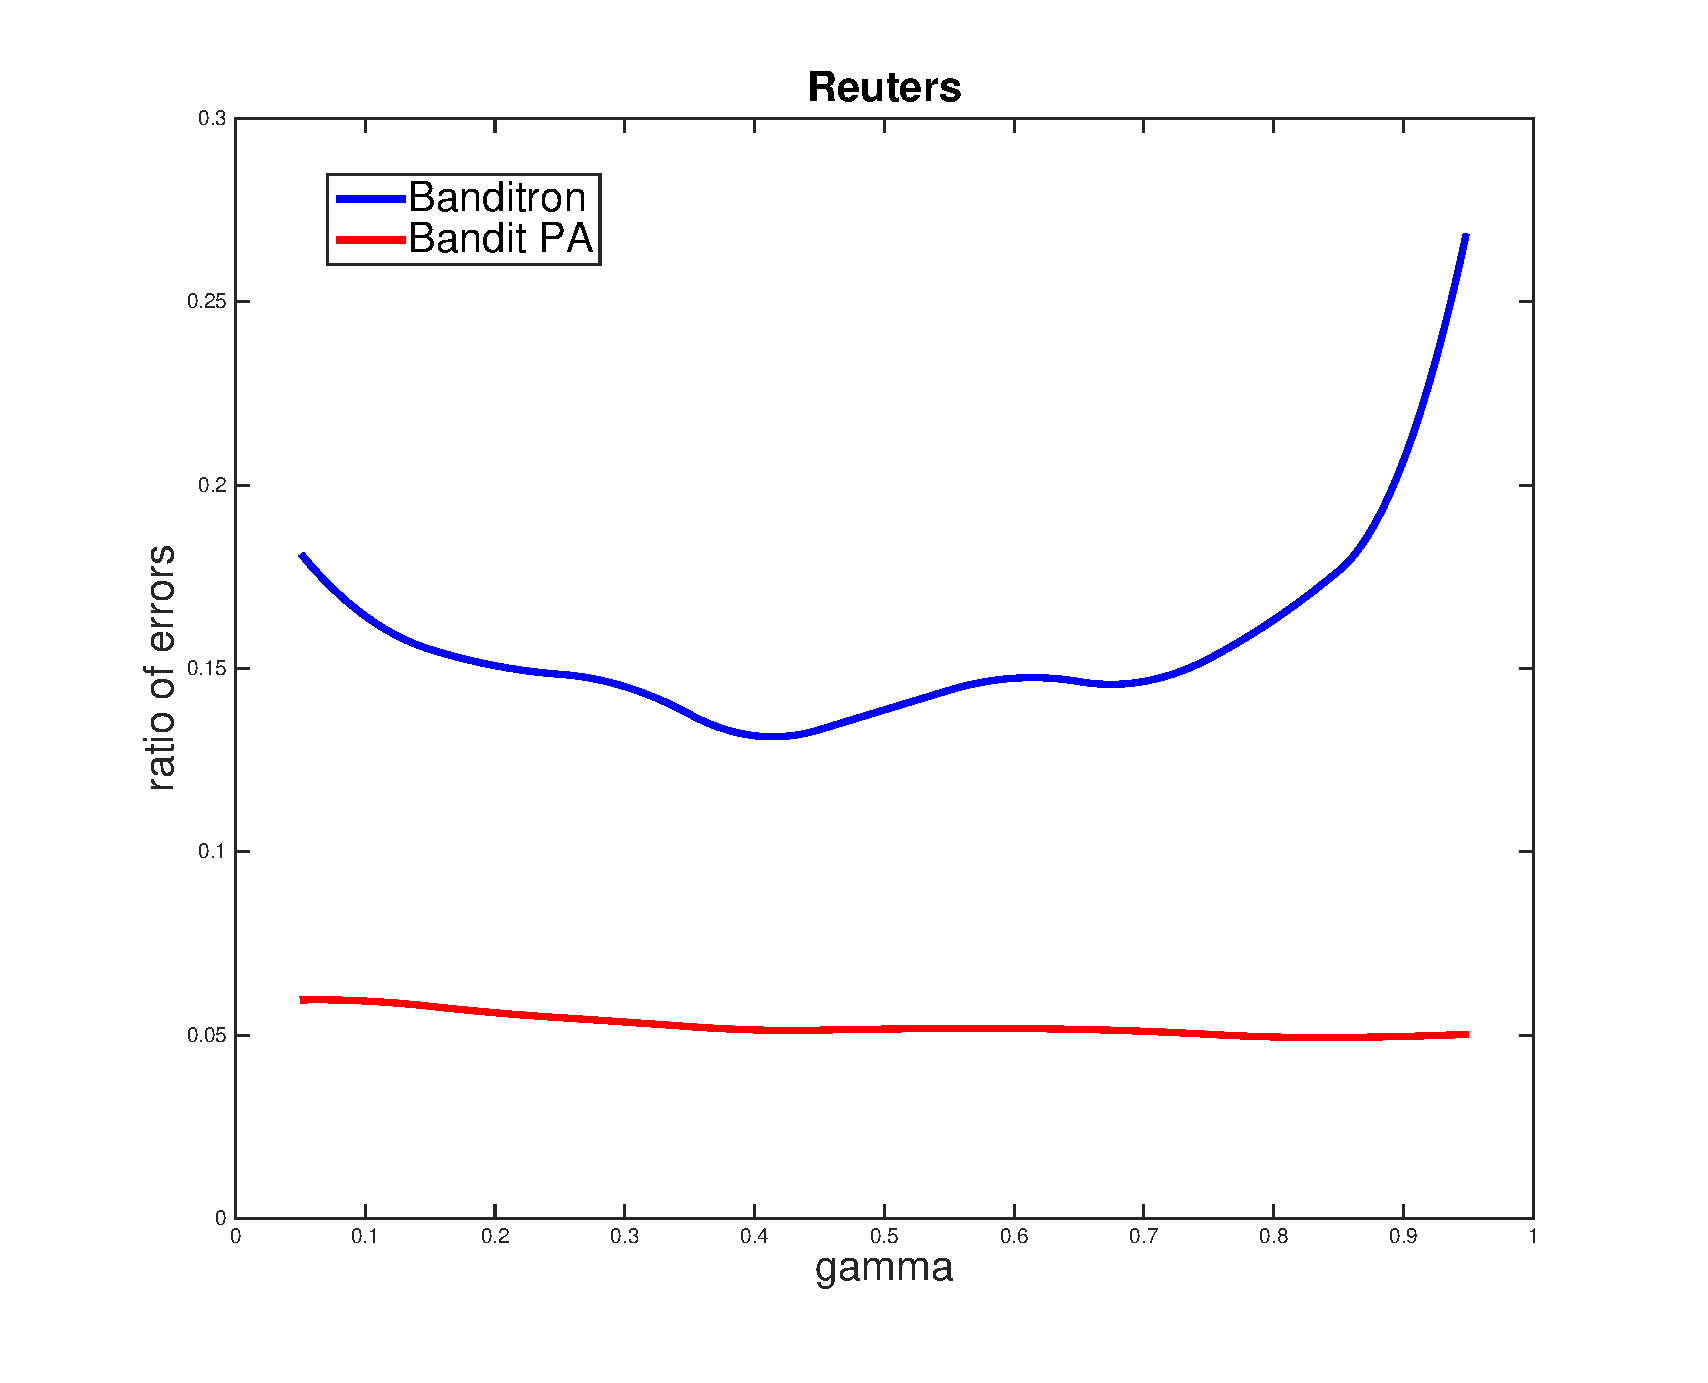
\includegraphics[scale = 0.4]{fig05/mc/Reuters_gamma.eps}}
\caption{Average error of Banditron and BPA for parameter's value $\gamma$ on the data set of Reuters.}
\label{pic:BPARCVerr}
\end{figure}

\begin{figure}[h!]
\label{pic:BPARCVerr}
\centerline{
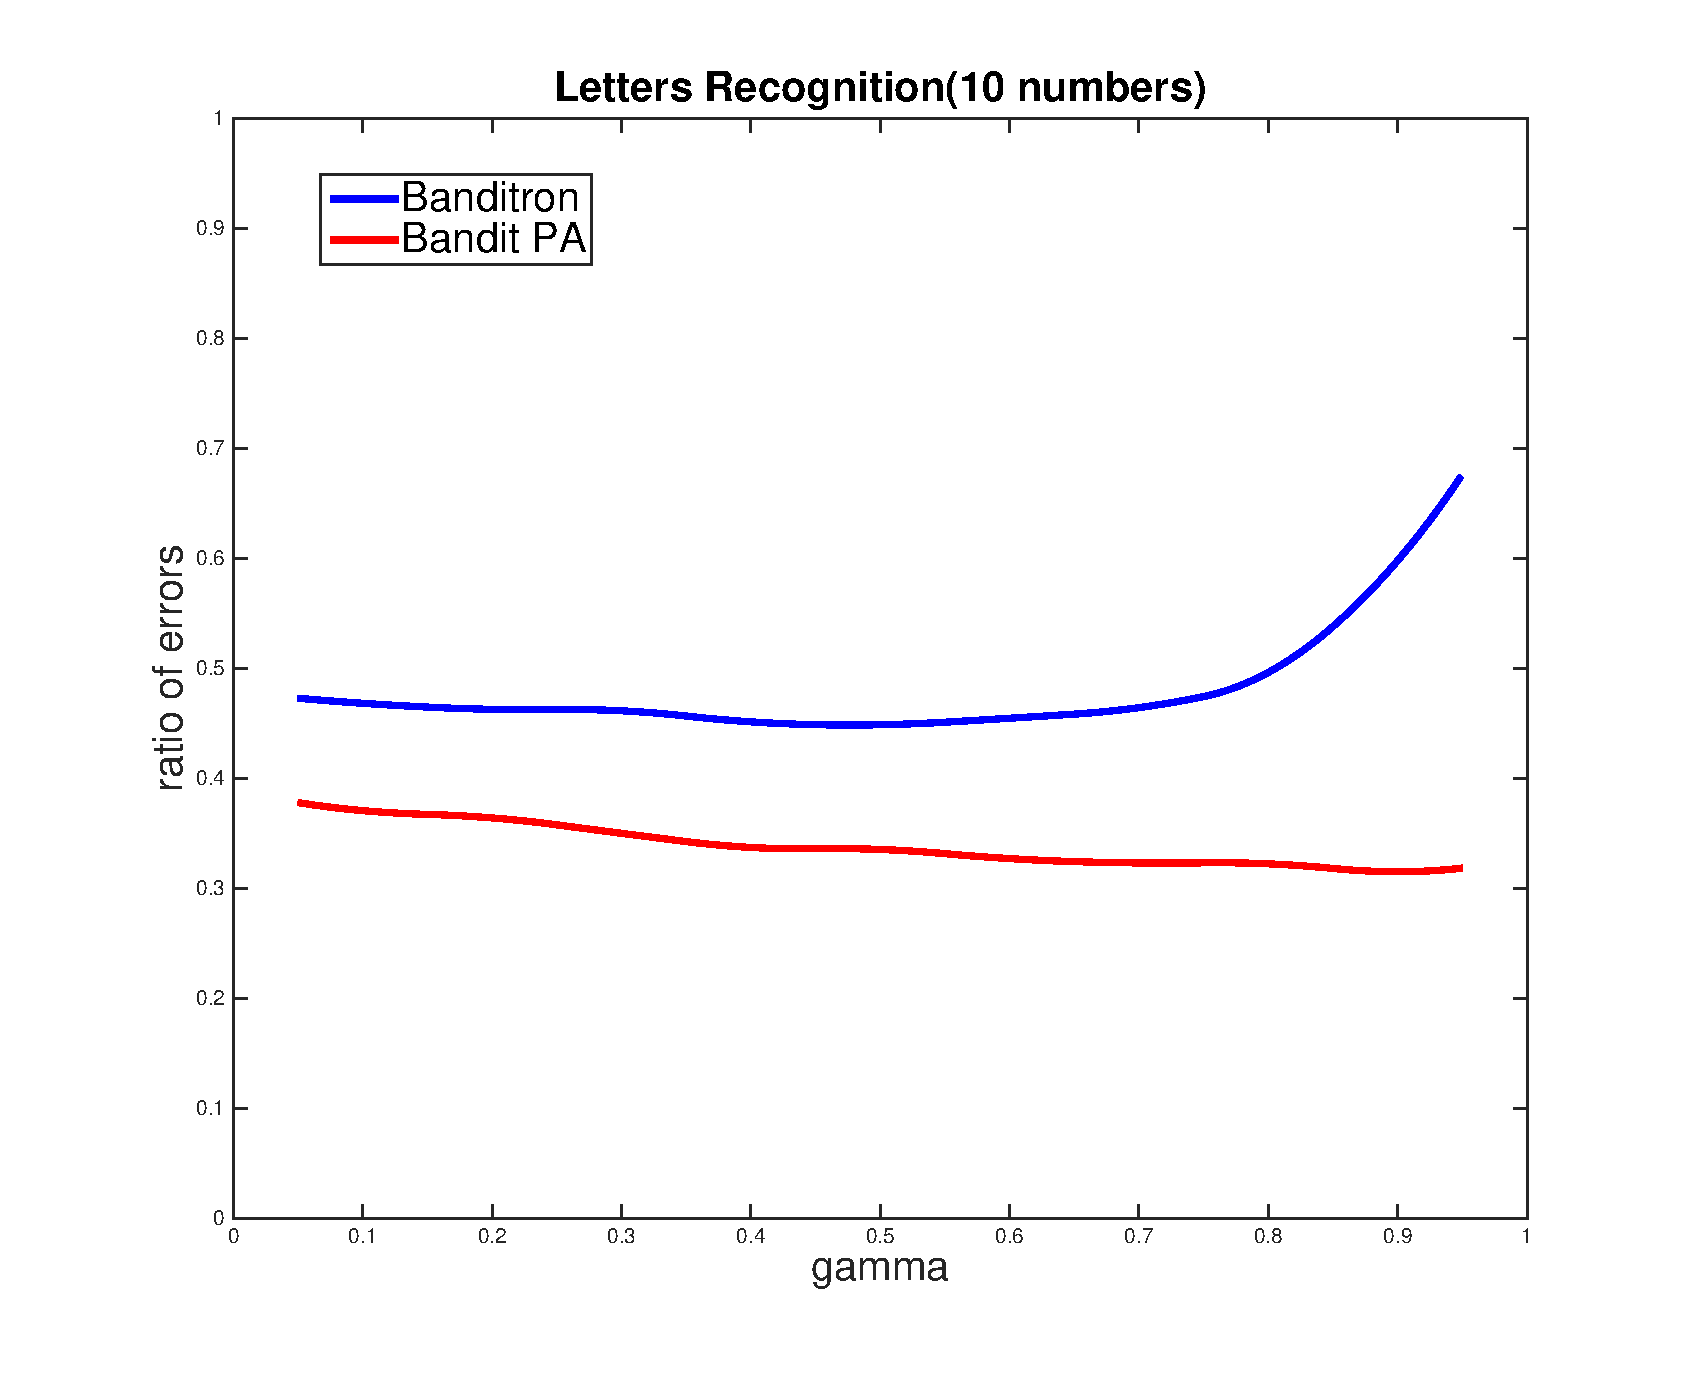
\includegraphics[scale = 0.4]{fig05/mc/10LR_gamma.eps}}
\caption{Average error of Banditron and BPA for parameter's value $\gamma$ on the data set of Letter Recognition.}
\end{figure}

\subsection{Conclusion}
\label{subsec:BPAC}
In this section, we proposed a novel algorithm for online multiclass with bandit feedback. By the advantage of PA max-margin principle, BPA appears effective to address the bandit online learning setting. Its main advantage is its linear complexity in space that allows to deal with high dimensional data sets and a large number of classes, on the contrary to second-order methods. The practicability of this algorithm is verified theoretically by showing a competitive loss bound.

Moreover, experimental evaluation shows that BPA performs better than other algorithms on some real sets, even better than the algorithms with full feedback on the data sets non-separable.
In the next section, we will take BPA to deal with data sets non-linear by combining the Kernel method. 